% Options for packages loaded elsewhere
\PassOptionsToPackage{unicode}{hyperref}
\PassOptionsToPackage{hyphens}{url}
%
\documentclass[
]{article}
\usepackage{amsmath,amssymb}
\usepackage{lmodern}
\usepackage{setspace} % add line to default template
\setstretch{1.2}      % add line to default template
\usepackage{iftex}
\ifPDFTeX
  \usepackage[T1]{fontenc}
  \usepackage[utf8]{inputenc}
  \usepackage{textcomp} % provide euro and other symbols
\else % if luatex or xetex
  \usepackage{unicode-math}
  \defaultfontfeatures{Scale=MatchLowercase}
  \defaultfontfeatures[\rmfamily]{Ligatures=TeX,Scale=1}
\fi
%% Support for zero-width non-joiner characters.
\makeatletter
\def\zerowidthnonjoiner{%
  % Prevent ligatures and adjust kerning, but still support hyphenating.
  \texorpdfstring{%
    \textormath{\nobreak\discretionary{-}{}{\kern.03em}%
      \ifvmode\else\nobreak\hskip\z@skip\fi}{}%
  }{}%
}
\makeatother
\ifPDFTeX
  \DeclareUnicodeCharacter{200C}{\zerowidthnonjoiner}
\else
  \catcode`^^^^200c=\active
  \protected\def ^^^^200c{\zerowidthnonjoiner}
\fi
%% End of ZWNJ support
% Use upquote if available, for straight quotes in verbatim environments
\IfFileExists{upquote.sty}{\usepackage{upquote}}{}
\IfFileExists{microtype.sty}{% use microtype if available
  \usepackage[]{microtype}
  \UseMicrotypeSet[protrusion]{basicmath} % disable protrusion for tt fonts
}{}
\makeatletter
\@ifundefined{KOMAClassName}{% if non-KOMA class
  \IfFileExists{parskip.sty}{%
    \usepackage{parskip}
  }{% else
    \setlength{\parindent}{0pt}
    \setlength{\parskip}{6pt plus 2pt minus 1pt}}
}{% if KOMA class
  \KOMAoptions{parskip=half}}
\makeatother
\usepackage{xcolor}
\IfFileExists{xurl.sty}{\usepackage{xurl}}{} % add URL line breaks if available
\IfFileExists{bookmark.sty}{\usepackage{bookmark}}{\usepackage{hyperref}}
\hypersetup{
  pdftitle={تحلیل داده‌های پیمایش ارزش‌های جهانی},
  pdfauthor={بهمن اجدری},
  hidelinks,
  pdfcreator={LaTeX via pandoc}}
\urlstyle{same} % disable monospaced font for URLs
\usepackage{longtable,booktabs,array}
\usepackage{calc} % for calculating minipage widths
% Correct order of tables after \paragraph or \subparagraph
\usepackage{etoolbox}
\makeatletter
\patchcmd\longtable{\par}{\if@noskipsec\mbox{}\fi\par}{}{}
\makeatother
% Allow footnotes in longtable head/foot
\IfFileExists{footnotehyper.sty}{\usepackage{footnotehyper}}{\usepackage{footnote}}
\makesavenoteenv{longtable}
\setlength{\emergencystretch}{3em} % prevent overfull lines
\providecommand{\tightlist}{%
  \setlength{\itemsep}{0pt}\setlength{\parskip}{0pt}}
\setcounter{secnumdepth}{-\maxdimen} % remove section numbering
\usepackage{amsmath}
\usepackage{booktabs}
\usepackage{caption}
\usepackage{longtable}
\usepackage{array}
\usepackage{multirow}
\usepackage{wrapfig}
\usepackage{float}
\usepackage{colortbl}
\usepackage{pdflscape}
\usepackage{tabu}
\usepackage{threeparttable}
\usepackage{threeparttablex}
\usepackage[normalem]{ulem}
\usepackage{makecell}
\usepackage{xcolor}
\ifLuaTeX
  \usepackage{selnolig}  % disable illegal ligatures
\fi

\title{تحلیل داده‌های پیمایش ارزش‌های جهانی}
\usepackage{etoolbox}
\makeatletter
\providecommand{\subtitle}[1]{% add subtitle to \maketitle
  \apptocmd{\@title}{\par {\large #1 \par}}{}{}
}
\makeatother
\subtitle{موج هفتم}
\author{بهمن اجدری}
\date{آبان ۱۴۰۱}

% ...................................................................... %
%
%               Add MPI Custom Template For Long Reprt
%
% ...................................................................... %
\usepackage{float}

% ...................................................................... %
% Load Packages
% tables requirement kableExtra packages2
% TODO: table striped dont work

% ...................................................................... %
% Add MPI Colors

% Colors extract from Max-Planck Society CD Manula
% https://docplayer.org/2328711-Max-planck-institut-das-erscheinungsbild-der-max-planck-gesellschaft-4-ueberarbeitete-auflage.html
\usepackage{xcolor}

\definecolor{MPIGreen}{HTML}{116656}
\definecolor{MPIGray}{HTML}{DDDED6}
\definecolor{MPIBlue}{HTML}{009EE2}
\definecolor{MPIRed}{HTML}{E90649}
\definecolor{MPILightBlue}{HTML}{40BDE8}
\definecolor{MPIOrange}{HTML}{FF7300}
\definecolor{MPIYellow}{HTML}{FFCE09}
\definecolor{MPIPink}{HTML}{FA9FCC}
\definecolor{MPILightGreen}{HTML}{62BD19}
\definecolor{MPILivingCoral}{HTML}{FC766A}
\definecolor{MPIPacificCoast}{HTML}{5B84B1}

% set titlepage top, bottom, text and rule color

\definecolor{titlepageTopColor}{HTML}{534B3E}


\definecolor{titlepageBottomColor}{HTML}{F8D940}


\definecolor{titlepageTextColor}{HTML}{F8D940}

\definecolor{titlepageAuthorTextColor}{HTML}{534B3E}


\definecolor{titlePageColor}{HTML}{009EE2}

\definecolor{titlePageRuleColor}{HTML}{ffffff}

\definecolor{pageBackgroundColor}{HTML}{ffffff}

\definecolor{bannerColor}{HTML}{40BDE8}

\definecolor{bannerTextColor}{HTML}{000000}

\definecolor{chapterTitleColor}{HTML}{000000}

% Set Initial Values

\def\titlepageRuleHeight{10}


\def\titleVjust{260}

\def\titleHjust{-40}


\def\authorVjust{-320}

\def\authorHjust{-40}


\def\logoPrimarySize{0.126}

\def\logoSecondarySize{0.126}

\def\bannerLogoSize{0.06}


% end of color and value definition
%......................................................................%

%......................................................................%
% set default hold position of figure and table
\makeatletter
  \providecommand*\setfloatlocations[2]{\@namedef{fps@#1}{#2}}
\makeatother
\setfloatlocations{figure}{H}
\setfloatlocations{table}{H}
%......................................................................%


%......................................................................%
% Add Main Fonts

% \usepackage{fontspec}


% define Vazir font for title
\newfontfamily\Vazir[
  Path=src/fonts/,
  LetterSpace=2.0,
  WordSpace={10,0,0},
  HyphenChar=None,
  PunctuationSpace=WordSpace
  ]{Vazir-Light-FD.ttf}
\newfontfamily\VazirCode[Path = src/fonts/]{Vazir-Code.ttf}


%......................................................................%
% add colored box environments

\usepackage[most]{tcolorbox}
\usepackage{awesomebox}

\newtcolorbox{info-box}{colback=cyan!5!white,arc=0pt,outer arc=0pt,colframe=cyan!60!black}
\newtcolorbox{warning-box}{colback=orange!5!white,arc=0pt,outer arc=0pt,colframe=orange!80!black}
\newtcolorbox{error-box}{colback=red!5!white,arc=0pt,outer arc=0pt,colframe=red!75!black}

% Think
\newenvironment{rmdThink}{
	\vspace*{0.5\baselineskip}
    \par\noindent
    \begin{tcolorbox}[enhanced, title={\large{\color{white}بیشتر بدانیم }},colback=MPIGreen!10!white, colframe=MPIGreen]
    \itshape
}{
    \end{tcolorbox}
    \par\ignorespacesafterend
}
\newtcolorbox{rmdthink}{colback=MPIGreen!10!white,colframe=MPIGreen,coltext=black,leftrule= 2mm,rightrule=0.5mm,bottomrule=0.5mm,toprule=0.5mm, boxsep=0.5pt,arc=2pt}

% Note
\newenvironment{rmdNote}{
	\vspace*{0.5\baselineskip}
    \par\noindent
    \begin{tcolorbox}[enhanced, title={\large{\color{white}توجه}},colback=MPIRed!10!white, colframe=MPIRed]
    \itshape
}{
    \end{tcolorbox}
    \par\ignorespacesafterend
}
\newtcolorbox{rmdnote}{colback=MPIRed!10!white,colframe=MPIRed,coltext=black,leftrule= 2mm,rightrule=0.5mm,bottomrule=0.5mm,toprule=0.5mm, boxsep=0.5pt,arc=2pt}

% Tip
\newenvironment{rmdTip}{
	\vspace*{0.5\baselineskip}
    \par\noindent
    \begin{tcolorbox}[enhanced, title={\large{\color{white}نکته}},colback=MPILightGreen!10!white, colframe=MPILightGreen]
    \itshape
}{
    \end{tcolorbox}
    \par\ignorespacesafterend
}
\newtcolorbox{rmdtip}{colback=MPILightGreen!10!white,colframe=MPILightGreen,coltext=black,leftrule= 2mm,rightrule=0.5mm,bottomrule=0.5mm,toprule=0.5mm, boxsep=0.5pt,arc=2pt}

% warning
\newenvironment{rmdWarning}{
	\vspace*{0.5\baselineskip}
    \par\noindent
    \begin{tcolorbox}[enhanced, title={\large{\color{white}هشدار}},colback=MPIOrange!10!white, colframe=MPIOrange]
    \itshape
}{
    \end{tcolorbox}
    \par\ignorespacesafterend
}
\newtcolorbox{rmdwarning}{colback=MPIOrange!10!white,colframe=MPIOrange,coltext=black,leftrule= 2mm,rightrule=0.5mm,bottomrule=0.5mm,toprule=0.5mm, boxsep=0.5pt,arc=2pt}

% todo
\newenvironment{rmdTodo}{
	\vspace*{0.5\baselineskip}
    \par\noindent
    \begin{tcolorbox}[enhanced, title={\large{\color{white}برای انجام}},colback=MPIBlue!10!white, colframe=MPIBlue]
    \itshape
}{
    \end{tcolorbox}
    \par\ignorespacesafterend
}
\newtcolorbox{rmdtodo}{colback=MPIBlue!10!white,colframe=MPIBlue,coltext=black,leftrule= 2mm,rightrule=0.5mm,bottomrule=0.5mm,toprule=0.5mm, boxsep=0.5pt,arc=2pt}



\newtcbtheorem[auto counter,number within=section]{Theorem}{قضیه}{%
                lower separated=false,fonttitle=\bfseries,
                colback=MPIGreen!10!white,colframe=MPIGreen,
                colbacktitle=MPIGreen, coltitle=white,
                enhanced,attach boxed title to top right={xshift=-0.5cm,yshift=-2mm}
                }{thm}

\newtcbtheorem[auto counter,number within=section]{Definition}{تعریف}{%
                lower separated=false,fonttitle=\bfseries,
                colback=MPILightGreen!10!white,colframe=MPILightGreen,
                colbacktitle=MPILightGreen, coltitle=white,
                enhanced,attach boxed title to top right={xshift=-0.5cm,yshift=-2mm}
                }{defn}

\newtcbtheorem[auto counter,number within=section]{Lemma}{لم}{%
                lower separated=false,fonttitle=\bfseries,
                colback=MPILightBlue!10!white,colframe=MPILightBlue,
                colbacktitle=MPILightBlue, coltitle=white,
                enhanced,attach boxed title to top right={xshift=-0.5cm,yshift=-2mm}
                }{lem}

\newtcbtheorem[auto counter,number within=section]{Corollary}{نتیجه}{%
                lower separated=false,fonttitle=\bfseries,
                colback=MPIBlue!10!white,colframe=MPIBlue,
                colbacktitle=MPIBlue, coltitle=white,
                enhanced,attach boxed title to top right={xshift=-0.5cm,yshift=-2mm}
                }{cor}

\newtcbtheorem[auto counter,number within=section]{Proposition}{گزاره}{%
                lower separated=false,fonttitle=\bfseries,
                colback=MPIYellow!10!white,colframe=MPIYellow,
                colbacktitle=MPIYellow, coltitle=white,
                enhanced,attach boxed title to top right={xshift=-0.5cm,yshift=-2mm}
                }{prop}

\newtcbtheorem[auto counter,number within=section]{Exercise}{تمرین}{%
                lower separated=false,fonttitle=\bfseries,
                colback=MPIRed!10!white,colframe=MPIRed,
                colbacktitle=MPIRed, coltitle=white,
                enhanced,attach boxed title to top right={xshift=-0.5cm,yshift=-2mm}
                }{exer}

\newtcbtheorem[auto counter,number within=section]{Example}{مثال}{%
                lower separated=false,fonttitle=\bfseries,
                colback=MPIOrange!10!white,colframe=MPIOrange,
                colbacktitle=MPIOrange, coltitle=white,
                enhanced,attach boxed title to top right={xshift=-0.5cm,yshift=-2mm}
                }{exam}

\newtcbtheorem[auto counter,number within=section]{Remark}{تذکر}{%
                lower separated=false,fonttitle=\bfseries,
                colback=MPIPink!10!white,colframe=MPIPink,
                colbacktitle=MPIPink, coltitle=white,
                enhanced,attach boxed title to top right={xshift=-0.5cm,yshift=-2mm}
                }{rmk}


\newtcbtheorem[auto counter,number within=section]{Proof}{اثبات}{%
                lower separated=false,fonttitle=\bfseries,
                colback=MPILivingCoral!10!white,colframe=MPILivingCoral,
                colbacktitle=MPILivingCoral, coltitle=white,
                enhanced,attach boxed title to top right={xshift=-0.5cm,yshift=-2mm}
                }{pr}

\newtcbtheorem[auto counter,number within=section]{Solution}{جواب}{%
                lower separated=false,fonttitle=\bfseries,
                colback=MPIPacificCoast!10!white,colframe=MPIPacificCoast,
                colbacktitle=MPIPacificCoast, coltitle=white,
                enhanced,attach boxed title to top right={xshift=-0.5cm,yshift=-2mm}
                }{sol}


\newenvironment{rmdexer}{
    \par\noindent
    \textbf{\color{MPIRed}Exercise} \itshape
}{\par}

\newenvironment{rmdsol}{
    \par\noindent
    \textbf{\color{MPIPacificCoast}Solution} \itshape
}{\par}


%......................................................................%
% add packages for title page

\definecolor{rcolor}{HTML}{2165B6}
\definecolor{rconsole}{HTML}{7E7E7E}

\newtcolorbox{rmdconsole}{
  enhanced,
  boxrule=0pt,
  colframe=rconsole,
  borderline west={4pt}{0pt}{rconsole},
  colback=rconsole!5!white,
  sharp corners
  }
\newtcolorbox{rmdcode}{
  enhanced,
  boxrule=0pt,
  colframe=rcolor,
  borderline west={4pt}{0pt}{rcolor},
  colback=rcolor!5!white,
  sharp corners
  }

\BeforeBeginEnvironment{verbatim}{
\begin{rmdconsole}
\begin{LTR}
}
\AfterEndEnvironment{verbatim}{
\end{LTR}
\end{rmdconsole}
}

\BeforeBeginEnvironment{Highlighting}{
\begin{rmdcode}
\begin{LTR}
\VazirCode
}
\AfterEndEnvironment{Highlighting}{
\end{LTR}
\end{rmdcode}
}


\definecolor{shadecolor}{HTML}{ffffff}

% Add quote section
\definecolor{quotecolor}{HTML}{989898}

\newtcolorbox{rmdquote}{
  enhanced,
  boxrule=0pt,
  colframe=quotecolor,
  borderline west={4pt}{0pt}{quotecolor},
  colback=quotecolor!15!white,
  sharp corners
  }
\BeforeBeginEnvironment{quote}{\begin{rmdquote}}
\AfterEndEnvironment{quote}{\end{rmdquote}}

% prevent vertically justifying the contents
\raggedbottom


%......................................................................%
% add packages for title page

\usepackage{tikz}

\usepackage[margin=1.5cm,includehead=true,includefoot=true,centering]{geometry}

% ----------------------------------------------------------------------------- %
%                                   Set Geometry                                %
% ----------------------------------------------------------------------------- %

\makeatletter
\def\parsecomma#1,#2\endparsecomma{\def\page@x{#1}\def\page@y{#2}}
\tikzdeclarecoordinatesystem{page}{
    \parsecomma#1\endparsecomma
    \pgfpointanchor{current page}{north east}
    % Save the upper right corner
    \pgf@xc=\pgf@x%
    \pgf@yc=\pgf@y%
    % save the lower left corner
    \pgfpointanchor{current page}{south west}
    \pgf@xb=\pgf@x%
    \pgf@yb=\pgf@y%
    % Transform to the correct placement
    \pgfmathparse{(\pgf@xc-\pgf@xb)/2.*\page@x+(\pgf@xc+\pgf@xb)/2.}
    \expandafter\pgf@x\expandafter=\pgfmathresult pt
    \pgfmathparse{(\pgf@yc-\pgf@yb)/2.*\page@y+(\pgf@yc+\pgf@yb)/2.}
    \expandafter\pgf@y\expandafter=\pgfmathresult pt
}
\makeatother


% ---------------------------------------------------------------------------- %
% header and footer
% ---------------------------------------------------------------------------- %

\usepackage{fancyhdr}
\pagestyle{fancy}
\fancyhf{}
\fancyhead[R]{\leftmark}
\fancyfoot[R]{\thepage}
\renewcommand{\headrulewidth}{0.5pt}
% \renewcommand{\footrulewidth}{0.25pt}


% TODO: Add header and footer options
% \lhead{}
% \chead{}
% \rhead{}
% \lfoot{}
% \cfoot{}
% \rfoot{}


% ---------------------------------------------------------------------------- %
% Banner Page Header and Footer Style



% ---------------------------------------------------------------------------- %
% Add Page Background


% ---------------------------------------------------------------------------- %
% Add Page Background Color
\usepackage{eso-pic}
\newcommand\BackPage{%
\begin{tikzpicture}[remember picture,overlay]
\fill[pageBackgroundColor](current page.south west) rectangle (\paperwidth,\paperheight);
\end{tikzpicture}%
}
%......................................................................%
% Remove Blank Page after Table of Contents and between chapter


%----------------------------------------------------------------------------------------
% Chapter Design
\usepackage{titlesec}

\titleformat{\section}[block]
  {\huge\color{chapterTitleColor}}
  {\filright \textbf{\thesection}\vspace{1ex}}{12pt}
  {}
  [\titlerule]

\titleformat{\subsection}[block]
  {\Large\color{chapterTitleColor}}
  {\filright \textbf{\thesubsection}\vspace{1ex}}{12pt}
  {}
  []



%----------------------------------------------------------------------------------------
% Remove page number in toc and strange white first page

%......................................................................%
%
%               End of Modifications
%
%......................................................................%
\usepackage{newunicodechar}

% Solve Half Space in Latex
\newunicodechar{‌}{\hskip 0pt}  % U+200c THIN SPACE

\usepackage[%
fontsizescale=1,%
latinfontsizescale=0.9,%
mathfontsizescale=1.1%
]{xepersian}
\settextfont[Path = src/fonts/, Scale=1]{Parastoo-FD.ttf}



\begin{document}
%......................................................................%
%               Add Titlepage
%......................................................................%


\begin{titlepage}

%......................................................................%
%                         Max-Planck Society Design

\begin{tikzpicture}[remember picture,overlay]



% add title page top color
\fill[titlepageTopColor] (page cs:-1,0.25) rectangle (current page.north east);

% add title page bottom color
\fill[titlepageBottomColor] (current page.south west) rectangle (page cs:1,0.25);


% add white rule



%......................................................................%


%......................................................................%
%                         FullCover Color Page Design

%......................................................................%




% add main logo % TODO: add else
\node[inner sep=0pt] at (page cs:-0.672,0.795){
\includegraphics[height=\logoPrimarySize\paperheight]{src/icon/RTLNotes.png}};
% add secondary logo % TODO: add else
\node[inner sep=0pt] at (page cs:-0.672,-0.795){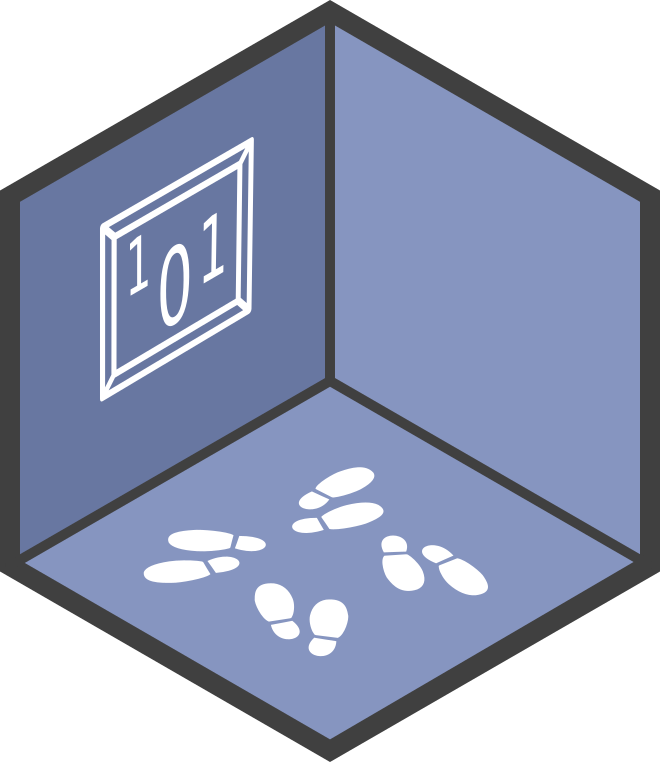
\includegraphics[height=\logoSecondarySize\paperheight]{src/icon/RWLogo.png}};

% add title and subtitle
\node[below,text width=\paperwidth,font=\color{titlepageTextColor}] at (page cs:0.0+\titleHjust,0.0+\titleVjust) {
\begin{flushright}
\begin{RTL}
    \Huge{تحلیل داده‌های پیمایش ارزش‌های جهانی}
  \vspace{0.3cm}
  
    \huge{موج هفتم}
  \vspace{0.3cm}
  
  % add bodoni font to date
    \vspace{0.3cm}
  \Large{آبان ۱۴۰۱}
  \vspace{0.3cm}
  
  \vspace{0.3cm}
    \Large{ تحلیل‌گر داده}
  \vspace{0.1cm}
  
    \large{تهران،ایران}
    \end{RTL}
  \end{flushright}
};

\node[below,text width=\paperwidth,font=\color{titlepageTextColor}] at (page cs:0.0+\authorHjust,0.0+\authorVjust) {

\begin{flushright}
\begin{RTL}
    \huge{\textcolor{titlepageAuthorTextColor}{بهمن اجدری}}
  \vspace{0.3cm}
  \end{RTL}
\end{flushright}

};

\end{tikzpicture}
\end{titlepage}
% \restoregeometry

% end design titlepage
%......................................................................%

%......................................................................%
% Add Page Background



% add these lines for simple report template
% end add



% add from eisvogel template



% Add Table of Contents
\thispagestyle{empty}
{
\setcounter{tocdepth}{3}
\tableofcontents
\newpage
}




\hypertarget{ux67eux6ccux645ux627ux6ccux634-ux627ux631ux632ux634ux647ux627ux6cc-ux62cux647ux627ux646ux6cc}{%
\section{پیمایش ارزش‌های
جهانی}\label{ux67eux6ccux645ux627ux6ccux634-ux627ux631ux632ux634ux647ux627ux6cc-ux62cux647ux627ux646ux6cc}}

در اواخر دهه ۷۰ میلادی دو استاد جامعه‌شناسی دانشگاه تیلبورگ در هلند در
فکر بررسی تاثیر تغییرات اقتصادی و فناوری بر زندگی روزمره انسان‌ها بودند.
آن‌ها می‌خواستند بدانند این رشد سریع اقتصاد و فناوری چه تاثیری بر جوامع
پیشرفته‌تر گذاشته و چگونه ارزش‌ها و نگرش‌های مردم را تغییر داده است. به
همین منظور پرسشنامه‌ای طراحی شد و در نزدیک به ۲۰ کشور پیشرفته اروپایی
توزیع شد تا بررسی شود مردم اروپا چطور فکر می‌کنند و چه چیزهایی برایشان
مهم است. صرف نظر از این نتایج پروژه، این پیمایش بزرگ نظر یک استاد علوم
سیاسی را هزاران کیلومتر آن‌طرف‌تر در میشیگان آمریکا به خود جلب کرد.\\
پروفسور رونالد اینگلهارت در اوایل دهه هشتاد میلادی مشغول کار مشابهی بود.
او مشغول نظریه پردازی در خصوص دلایل تغییرات سریع و ناگهانی چرخش‌های
فرهنگی، سیاسی و اجتماعی در اروپای غربی و آمریکای شمالی بود که با اطلاع
از پروژه دانشگاه تیلبورگ در هلند پیشنهاد توسعه سوالات پرسشنامه برای
دربرگرفتن طیف بیشتری از خصوصیات سیاسی، اجتماعی و رفتاری پاسخ‌دهندگان و
همچنین توسعه جغرافیایی محل توزیع پرسشنامه‌ها به ماورای مرزهای اروپا را
مطرح کرد. اینگلهارت با راه اندازی پروژه‌ای به نام پیمایش ارزش‌های جهانی در
سال ۱۹۸۱ یکی بزرگترین پروژه‌های دانشگاهی جهان در حوزه علوم اجتماعی را
کلید زد که تاکنون نیز ادامه دارد.\\
رونالد اینگلهارت (۲۰۲۱-۱۹۳۴)در طول دوران خود کاری دستاوردهای بزرگی باقی
گذاشت. مقالات و کتاب‌های متعددی از وی که بسیاری از آن‌ها منابع اصلی علوم
سیاسی و اجتماعی محسوب می‌شوند از میراث ماندگار اوست. اما شاید بزرگترین
خدمت او به علوم اجتماعی، داده‌های پرسشنامه‌ای است که با نظارت وی در ۱۲۰
کشور جهان (تقریبا ۹۰ درصد جمعیت جهان) در ۷ مقطع زمانی جمع‌آوری شده است.
این داده‌ها بصورت رایگان در اختیار مردم و جامعه دانشگاهی قرار گرفته است و
تا کنون در طیف وسیعی از شاخه‌های علوم اجتماعی مورد استفاده قرار گرفته
است. چند صدهزار نفری که در تمام دنیا مورد پرسش قرار گرفته‌اند امکان
مقایسه دیدگاه‌های مردم دنیا را در مکان‌های جغرافیایی مختلف را فراهم می‌کند.

\hypertarget{ux62fux627ux62fux647ux647ux627ux6cc-ux627ux6ccux631ux627ux646}{%
\subsection{داده‌های
ایران}\label{ux62fux627ux62fux647ux647ux627ux6cc-ux627ux6ccux631ux627ux646}}

از ۷ موج انجام شده در موسسه پیمایش ارزش‌های جهانی، ایرانیان در سه موج
چهارم، پنجم و هفتم حاضر هستند. دولت دهم ایران اجازه برگزاری موج ششم را
در ایران نداد. موج هفتم در ایران در سال ۱۳۹۹ انجام شده است و داده‌های آن
در سال ۱۴۰۰ منتشر شده است. لازم به ذکر است که موج هفتم به دلیل
محدودیت‌های همه‌گیری کرونا، فرایند جمع‌آوری و انتشار داده‌ها کمی بیشتر از حد
معمول طول کشیده است. داده‌های ایران (۱۵۰۰ پرسشنامه) برای جمعیت ایران معرف
است. به بیان دیگر تحلیل‌های مبتنی بر داده‌های پیمایش ارزش‌های جهانی قابل
تعمیم به کل جمعیت ایران است.\\
تعداد سوالات پرسشنامه ایران، ۲۹۰ سوال است. این سوالات عموما به صورت
مصاحبه حضوری از مخاطبین پرسیده شده. شرایط پاسخ به سوالات و زمان دقیق
پاسخ‌ها در فایل داده‌ها موجود است. پاسخ دهندگان به صورت تصادفی از جمعیت
کشور انتخاب شده‌اند و امکان دسترسی به هویت آن‌ها از طریق پرسشنامه
امکان‌پذیر نیست.

\hypertarget{ux646ux62dux648ux647-ux627ux633ux62aux641ux627ux62fux647-ux627ux632-ux62fux627ux62fux647}{%
\subsection{نحوه استفاده از
داده}\label{ux646ux62dux648ux647-ux627ux633ux62aux641ux627ux62fux647-ux627ux632-ux62fux627ux62fux647}}

داده‌های پیمایش جهانی در حوزه‌های مختلفی از جمله توسعه اقتصادی، توسعه
دموکراسی، دین، برابری جنسیتی، سرمایه اجتماعی و بهداشت عمومی قابل استفاده
است. این داده‌ها بر اساس پرسشنامه‌ای است که با جمع‌بندی پیشنهادهای اساتید
علوم اجتماعی در سراسر جهان که به موسسه پیمایش ارزش‌های جهانی ارائه می‌شود.
پرسشنامه هر کشور نیز از وب‌سایت موسسه قابل دسترسی است. لازم به ذکر است که
هر کشور می‌تواند تغییرات بسیار محدودی را در پرسشنامه ایجاد کند. این
تغییرات نباید برای بیشتر از ۱۲ سوال از کل سوالات موجود در پرسشنامه
باشد.\\
استفاده از این داده‌ها تنها برای مقاصد غیر انتفاعی مجاز است. در صورت
استفاده از این داده‌ها در مقالات و پایان‌نامه‌های دانشگاهی،ارجاع به داده‌ها
باید به صورتی که وب‌سایت موسسه آورده شده در بخش منابع مقاله یا پایان‌نامه
قرار‌ گیرد. برای نمونه اگر از موج ششم پیمایش برای کار تحقیقی استفاده
کرده‌اید باید به صورت زیر به آن ارجاع دهید:

\begin{quote}
Inglehart, R., C. Haerpfer, A. Moreno, C. Welzel, K. Kizilova, J.
Diez-Medrano, M. Lagos, P. Norris, E. Ponarin \& B. Puranen et
al.~(eds.). 2014. World Values Survey: Round Six - Country-Pooled
Datafile Version:
\url{https://www.worldvaluessurvey.org/WVSDocumentationWV6.jsp}. Madrid:
JD Systems Institute.
\end{quote}

\hypertarget{ux646ux62dux648ux647-ux62fux633ux62aux631ux633ux6cc-ux628ux647-ux62fux627ux62fux647ux647ux627}{%
\subsection{نحوه دسترسی به
داده‌ها}\label{ux646ux62dux648ux647-ux62fux633ux62aux631ux633ux6cc-ux628ux647-ux62fux627ux62fux647ux647ux627}}

تمام داده‌ها از وب‌سایت رسمی پیمایش ارزش‌های جهانی قابل دریافت است. داده‌ها
در انواع مختلفی قابل دسترس است که امکان استفاده از نرم‌افزار‌های مختلف از
جمله R و SPSS را فراهم می‌کند. داده‌ها به تفکیک هر موج و یا بصورت تجمیع
شده قابل دسترس است. همچنین می‌توانید داده‌های هر کشور را جداگانه و در
فرمت‌های داده مختلف را از سایت موسسه دریافت کنید.

\newpage

\hypertarget{ux645ux634ux62eux635ux627ux62a-ux67eux627ux633ux62eux6afux648ux6ccux627ux646}{%
\section{مشخصات
پاسخگویان}\label{ux645ux634ux62eux635ux627ux62a-ux67eux627ux633ux62eux6afux648ux6ccux627ux646}}

\begin{verbatim}
[1] "urban" "rural"
\end{verbatim}

\hypertarget{ux62cux646ux633ux6ccux62a-ux67eux627ux633ux62eux62fux647ux646ux62fux6afux627ux646}{%
\subsection{جنسیت
پاسخ‌دهندگان}\label{ux62cux646ux633ux6ccux62a-ux67eux627ux633ux62eux62fux647ux646ux62fux6afux627ux646}}

\begin{center}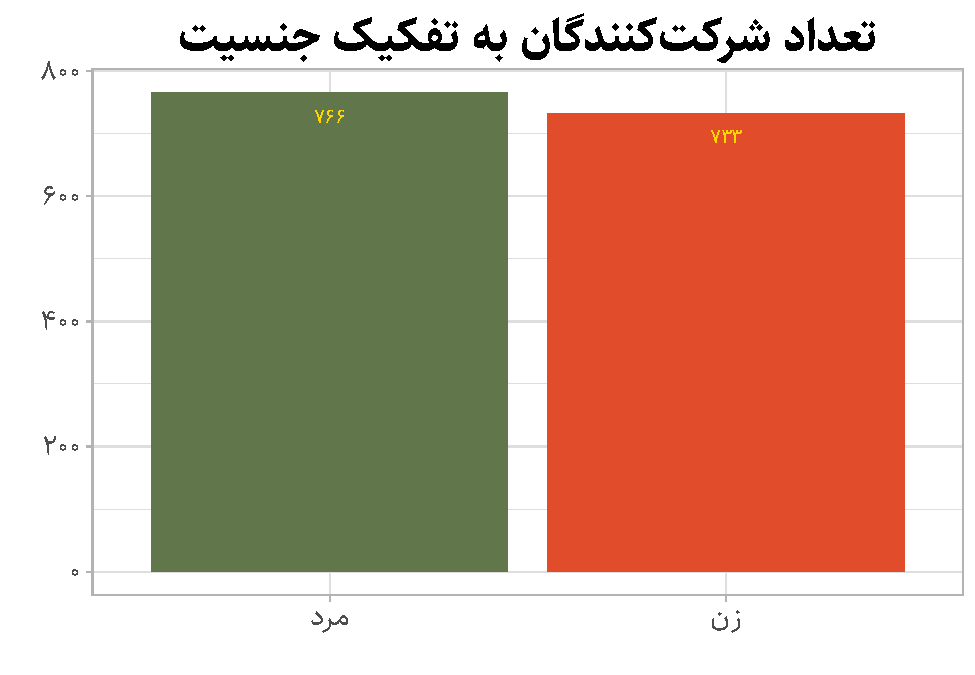
\includegraphics{figure/unnamed-chunk-3-1} \end{center}

\begin{longtable}[]{@{}lrl@{}}
\toprule
gender & n & pct \\
\midrule
\endhead
مرد & 766 & 51\% \\
زن & 733 & 49\% \\
\bottomrule
\end{longtable}

\hypertarget{ux633ux646-ux67eux627ux633ux62eux62fux647ux646ux62fux6afux627ux646}{%
\subsection{سن
پاسخ‌دهندگان}\label{ux633ux646-ux67eux627ux633ux62eux62fux647ux646ux62fux6afux627ux646}}

\begin{center}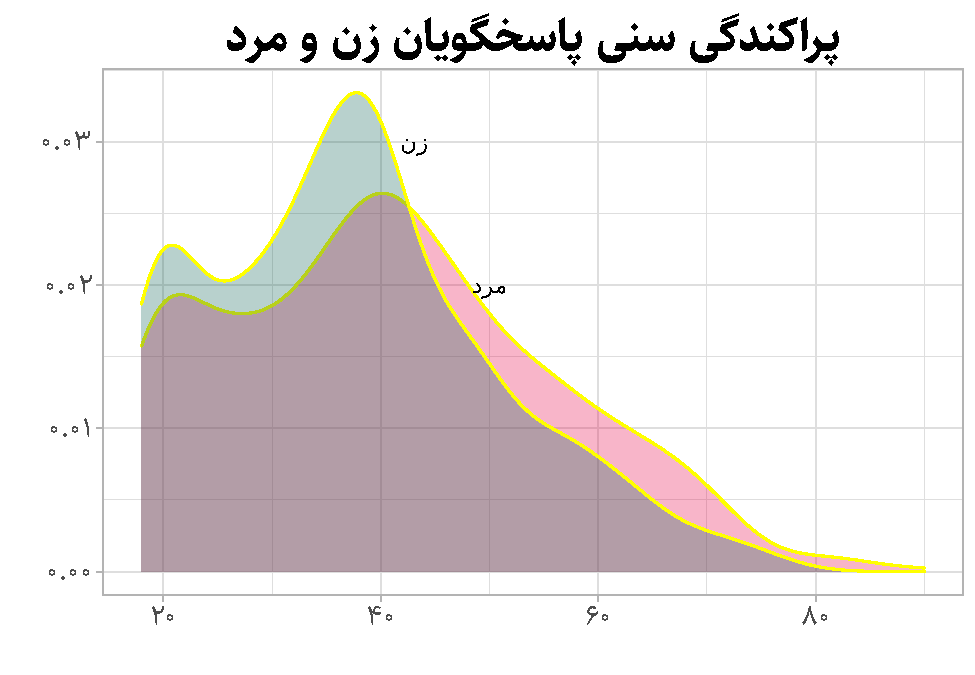
\includegraphics{figure/unnamed-chunk-5-1} \end{center}
\begin{longtable}{rrc}
\caption*{
{\large توزیع سنی پاسخ‌دهندگان} \\ 
{\small موج هفتم پیمایش ارزش‌های جهانی}
} \\ 
\toprule
درصد & فراوانی & سن \\ 
\midrule
28 & 420 & 18-29 \\ 
49 & 738 & 30-49 \\ 
23 & 341 & 50+ \\ 
\bottomrule
\end{longtable}

\hypertarget{ux62aux648ux632ux6ccux639-ux645ux6a9ux627ux646ux6cc-ux67eux627ux633ux62eux62fux647ux646ux62fux6afux627ux646}{%
\subsection{توزیع مکانی
پاسخ‌دهندگان}\label{ux62aux648ux632ux6ccux639-ux645ux6a9ux627ux646ux6cc-ux67eux627ux633ux62eux62fux647ux646ux62fux6afux627ux646}}

\begin{table}
\centering
\begin{tabular}[t]{>{\raggedright\arraybackslash}p{10em}>{\raggedleft\arraybackslash}p{10em}>{\raggedleft\arraybackslash}p{10em}}
\toprule
سن & فراوانی & درصد\\
\midrule
18-29 & 420 & 28\\
30-49 & 738 & 49\\
50+ & 341 & 23\\
\bottomrule
\end{tabular}
\end{table}

\begin{center}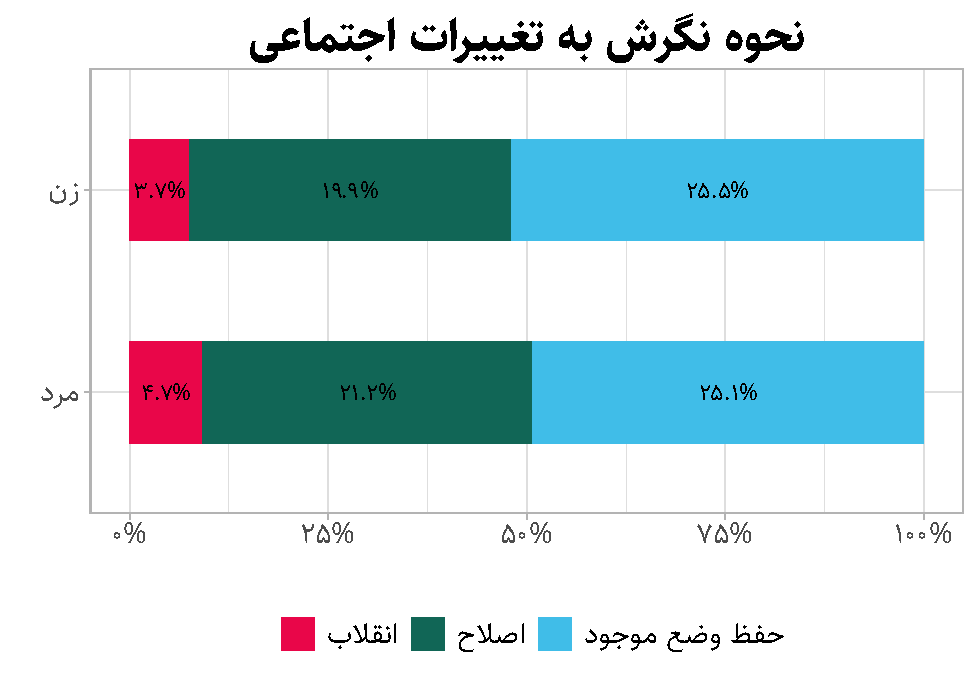
\includegraphics{figure/unnamed-chunk-8-1} \end{center}

\begin{verbatim}
# A tibble: 5 x 2
      t     n
  <dbl> <int>
1    -2     4
2    -1     6
3     1   858
4     2   293
5     3   338
\end{verbatim}

\end{document}
